
\textbf{Exercise 6. }\emph{Consider the Wiener (standard Brownian) process \( W(t) \)  in \( [0, 1] \).}
\begin{itemize}
  \item[\textit{(i)}] \emph{The property of independent increments states that, given \( t_{2} \geq t_{1} \geq s_{2} \geq s_{1} \geq 0 \), it holds that:}
        \[
        \mathbb{E}[(W(t_{2}) - W(t_{1}))(W(s_{2}) - W(s_{1}))] = \mathbb{E}[W(t_{2}) - W(t_{1})]\mathbb{E}[W(s_{2}) - W(s_{1})].
        \]
        \emph{From this property, show that the autocovariances are given by}
        \[
        \gamma(t, s) = \mathbb{E}[W(t)W(s)] = min(t,s)\quad \forall t,s\in [0,1].
        \]
        \item[\textit{(ii)}] \emph{Illustrate this property by simulating a Wiener process in \( [0 ,1] \) and making a plot of the sample estimate and the theoretical values of \( \gamma(t, 0.25) \) as a function of \( t \in [0, 1] \).}
\end{itemize}

\textit{Solution.}
\begin{itemize}
  \item[\textit{(i)}] Let \( t \geq s \). Using that \( W(t) = W(t) - W(s) + W(s) \) we may write the desired covariance as:
        \begin{equation}\label{eq:cov}
        \gamma(t, s) = \mathbb{E}[W(t)W(s)] = \mathbb{E}[(W(t) - W(s) + W(s))W(s)] = \mathbb{E}[(W(t) - W(s))W(s)] + \mathbb{E}[W(s)^{2}].
      \end{equation}
        Now, since $W(0)=0$, we note that \( W(s) = W(s) - W(0) \), and so:
        \[
        \mathbb{E}[(W(t) - W(s))W(s)] = \mathbb{E}[(W(t) - W(s))(W(s) - W(0))] = \mathbb{E}[W(t) - W(s)]\mathbb{E}[W(s)] = 0,
        \]
        where we have used the fact that the mean function is $0$, and the independence of the increments:
        \[
        W(t) - W(s) \perp W(s) - W(0) = W(s).
        \]
        Thus substituting back in Eq. \eqref{eq:cov}}, we arrive at:
        \[
        \gamma(t, s) = \mathbb{E}[W(s)^{2}] = Var[W(s)]=s = min(t, s).
        \]
        As both $t$ and $s$ were arbitrary, reversing their roles gives us the equality in the case $s\geq t$.

        \item[\textit{(ii)}] \emph{Illustrate this property by simulating a Wiener process in \( [0 ,1] \) and making a plot of the sample estimate and the theoretical values of \( \gamma(t, 0.25) \) as a function of \( t \in [0, 1] \).}

        We simulate $10^4$ Wiener processes in $[0,1]$, and we use them to estimate the sample covariance $\gamma(t, 0.25)$ for each $t$. We plot the theoretical values of these autocovariances against the estimated values, and the results are as follows:

        \begin{figure}[h!]
          \centering
          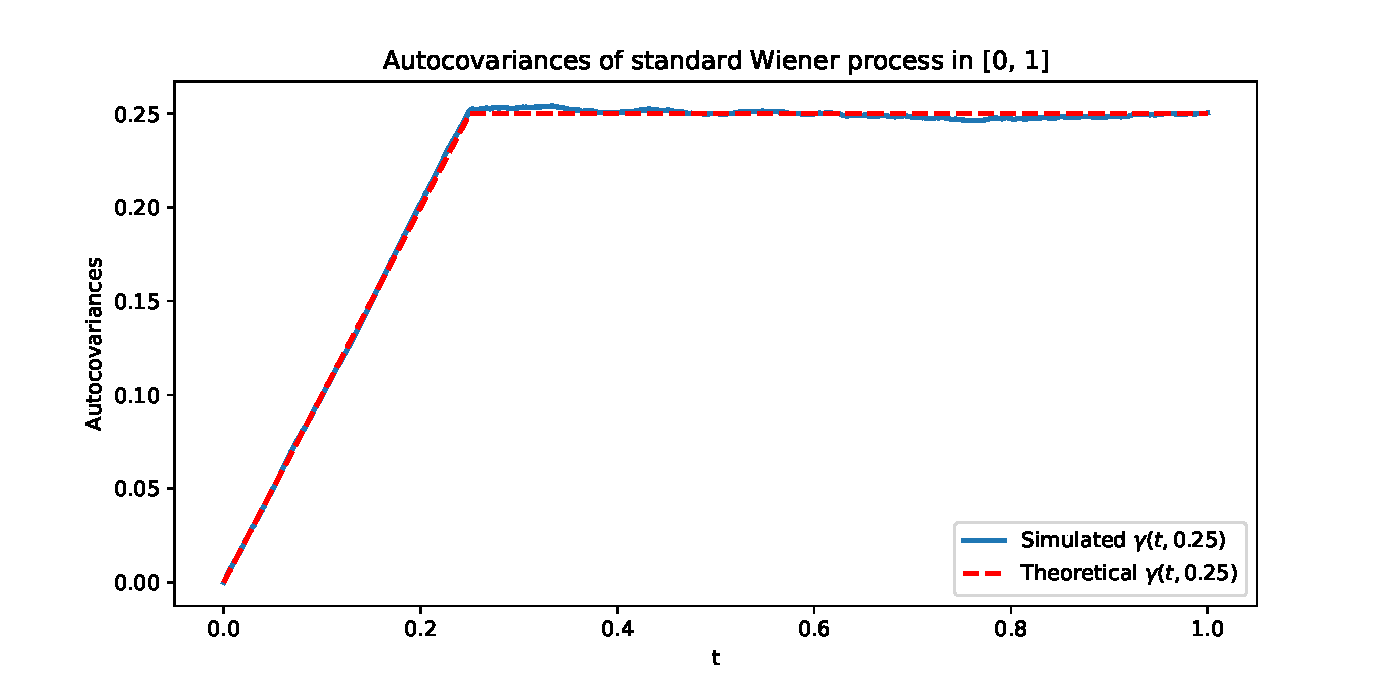
\includegraphics[width=.8\textwidth]{img/ex6.pdf}
        \end{figure}
        As we can see, the simulation confirms our calculations.\\
\end{itemize}
